\documentclass{standalone}
\usepackage{pgfplots}
\usepackage{lmodern}
\pgfplotsset{compat=1.17}

\begin{document}
	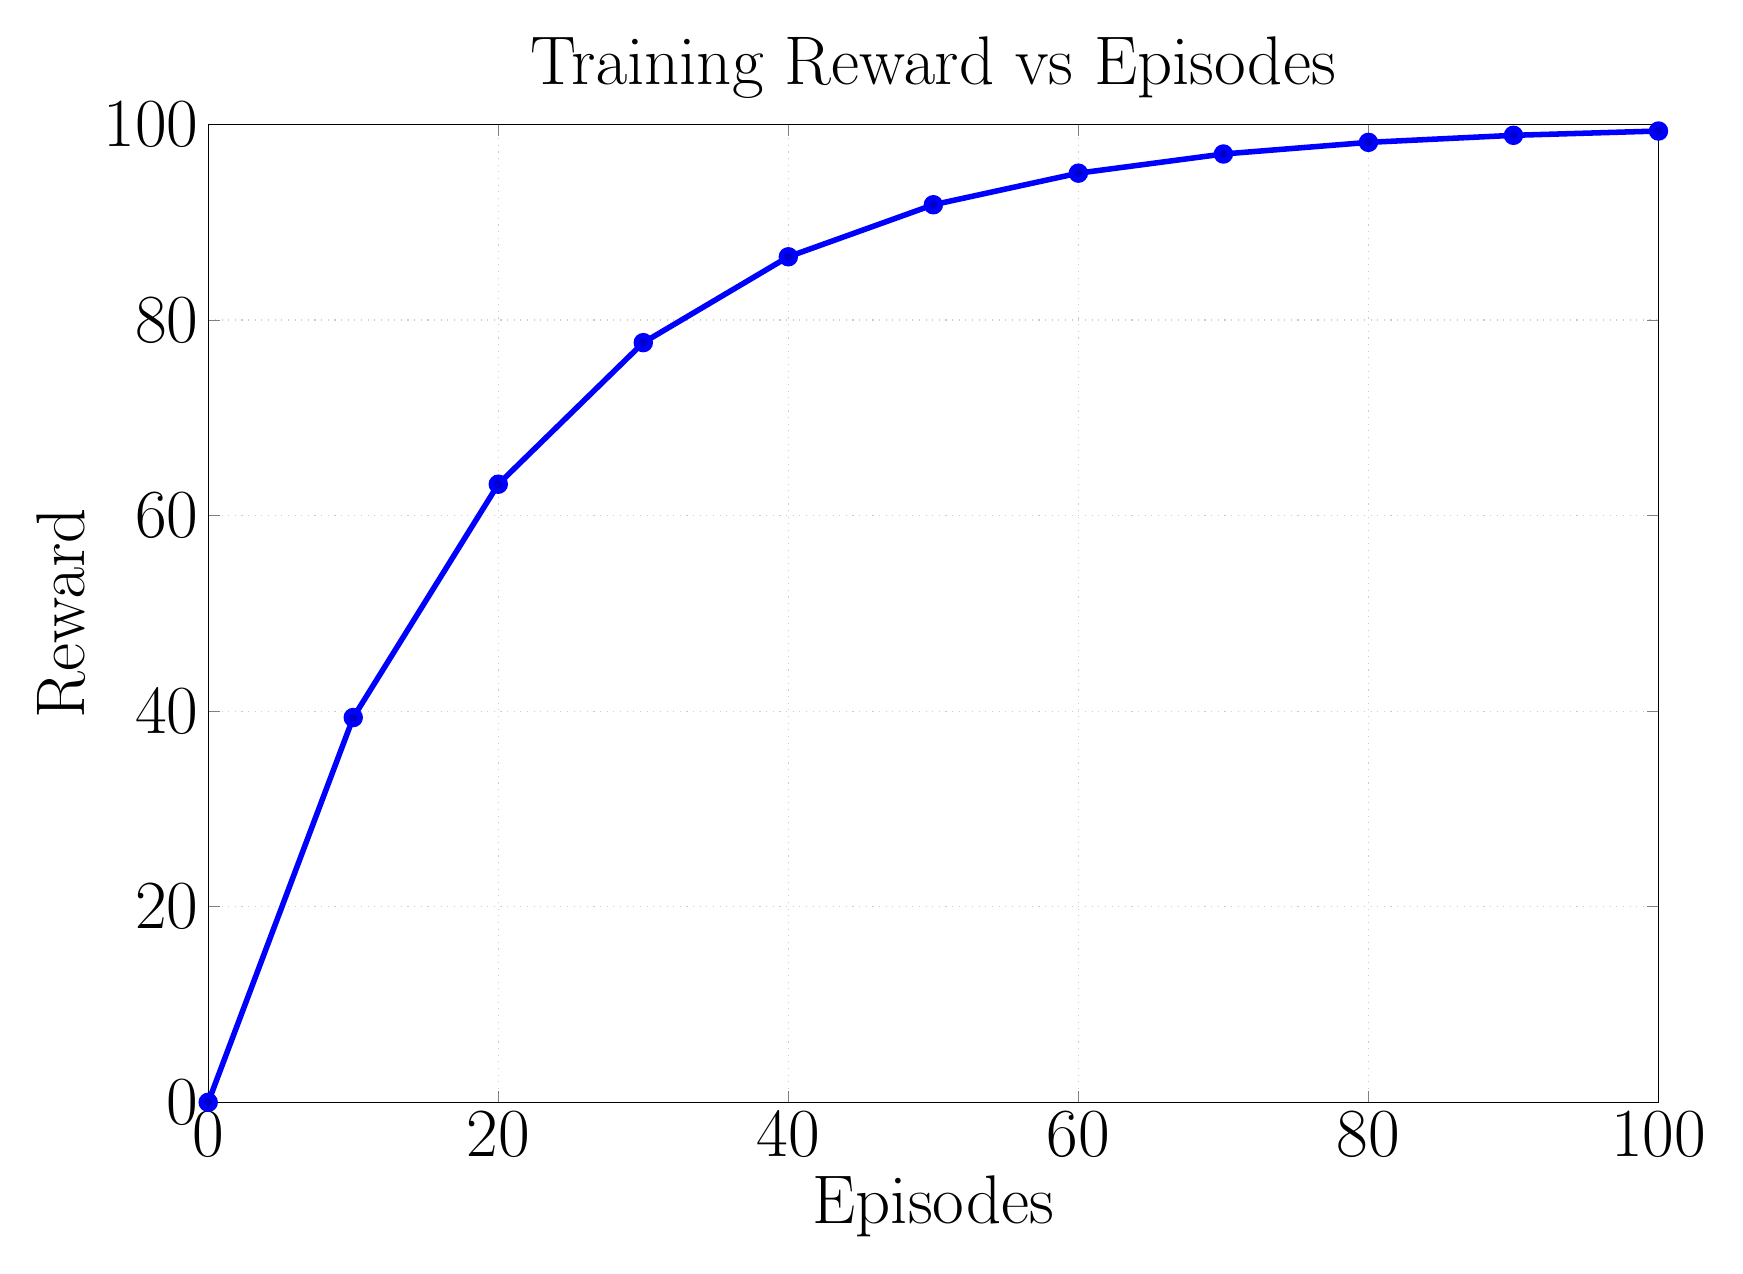
\begin{tikzpicture}
		\begin{axis}[
			width=20cm,
			height=14cm,
			tick label style={font=\fontsize{24}{28}\selectfont},
			label style={font=\fontsize{24}{28}\selectfont},
			title style={font=\fontsize{24}{28}\selectfont},
			xlabel={Episodes},
			ylabel={Reward},
			title={Training Reward vs Episodes},
			xmin=0, xmax=100,
			ymin=0, ymax=100,
			xtick={0,20,40,60,80,100},
			ytick={0,20,40,60,80,100},
			grid=both,
			grid style={dotted, gray!40},
		]
			
			\addplot+[mark=*, color=blue, line width=2pt, mark size=2.5pt] coordinates {
				(0,0)(10,39.35)(20,63.21)(30,77.69)(40,86.47)(50,91.79)(60,95.02)(70,96.98)(80,98.17)(90,98.89)(100,99.33)
			};
			
		\end{axis}
	\end{tikzpicture}
\end{document}
